\documentclass[a4paper,12pt]{article} % добавить leqno в [] для нумерации слева
\usepackage[a4paper,top=1.3cm,bottom=2cm,left=1.5cm,right=1.5cm,marginparwidth=0.75cm]{geometry}
%%% Работа с русским языком
\usepackage{cmap}					% поиск в PDF
\usepackage{mathtext} 				% русские буквы в фомулах
\usepackage[T2A]{fontenc}			% кодировка
\usepackage[utf8]{inputenc}			% кодировка исходного текста
\usepackage[english,russian]{babel}	% локализация и переносы

\usepackage{graphicx}

\usepackage{wrapfig}
\usepackage{tabularx}

\usepackage{hyperref}
\usepackage[rgb]{xcolor}
\hypersetup{
colorlinks=true,urlcolor=blue
}
\usepackage{multirow}
\usepackage{hhline}


%%% Дополнительная работа с математикой
\usepackage{amsmath,amsfonts,amssymb,amsthm,mathtools} % AMS
\usepackage{icomma} % "Умная" запятая: $0,2$ --- число, $0, 2$ --- перечисление

%% Номера формул
\mathtoolsset{showonlyrefs=true} % Показывать номера только у тех формул, на которые есть \eqref{} в тексте.

%% Шрифты
\usepackage{euscript}	 % Шрифт Евклид
\usepackage{mathrsfs} % Красивый матшрифт

%% Свои команды
\DeclareMathOperator{\sgn}{\mathop{sgn}}

%% Перенос знаков в формулах (по Львовскому)
\newcommand*{\hm}[1]{#1\nobreak\discretionary{}
{\hbox{$\mathsurround=0pt #1$}}{}}

\begin{document}
	
	\begin{center}
		{\huge \bf{Вопрос по выбору}}
	\end{center}
	\begin{center}
		{\huge Ламповый генератор высокочастотных колебаний}
	\end{center}

\section{Схема и принцип работы}

\noindent Генератор, схема которого представлена на рисунке, создает высокое напряжение (3-4 тысячи вольт) высокой частоты (около 5 МГц). Колебательный контур, определяющий частоту генератора, состоит из катушки $L_1$ и усилителя, собранного на лампе Л$_1$: часть энергии контура забирается этой катушкой, подается на сетку лампы, усиливается и через конденсатор $C_2$ подается обратно в контур. Цепочка $R_1 C_3$ обеспечивает отрицательное постоянное напряжение на сетке лампы, необходимое для ее нормальной работы. Дроссель разделяет участки цепи, где высокочастотное напряжение есть (анод лампы) и где его нет ("плюс" источника питания). Это происходит благодаря большому сопротивлению дросселя переменному току высокой частоты. Вторая сетка лампы соединена с анодом, в результате лампа работает как триод. Катушки $L_1, L_2, L_3$ идуктивно связаны и образуют высокочастотный трансформатор.

\medskip
\begin{center}

  \centering
  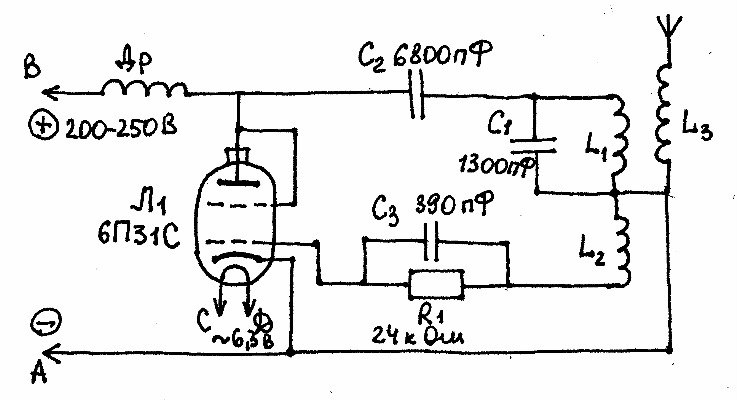
\includegraphics[scale={0.4}]{схема.jpg}

\end{center}

\noindent 

\section{Процесс изготовления}

\noindent Катушки будем наматывать вручную. $L_1$ и $L_2$ наматываются на общий циоиндрический каркас диаметром 3,5 см и длиной 7 см, изготовленный из картона. Первая катушка состоит из 6 витков медного провода диаметром 2-3 мм в эмалевой изоляции, расстояние между витками равно 1 см. Вторая содержит 10 витков провода в эмалевой изоляции диаметром 0,5 мм, намотанных вплотную. Катушка $L_3$ содержит 190 витков провода ПЭЛШО диаметром 0,4 мм, Она вставлена внутрь катушек $L_1$ и $L_2$. Дроссель содержит 70 витков провода диаметром 0,3 мм, намотанных в один слой на каркас диаметром 2,5 см.

\medskip

\noindent В специальной программе была разработана разметка печатной платы, после чего плата была фрезерована на станке Charly4U.

\medskip
\begin{center}

  \centering
  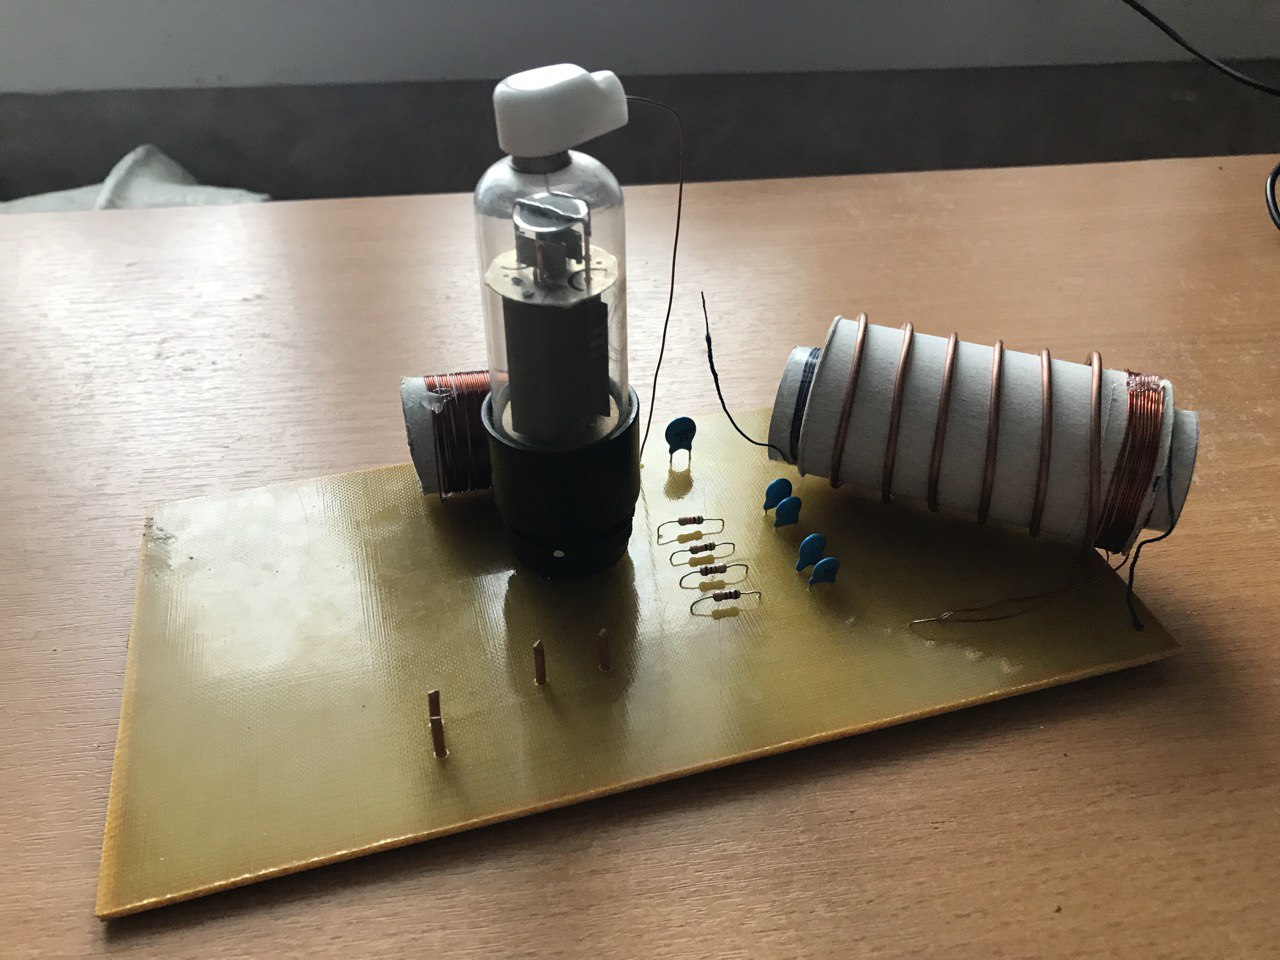
\includegraphics[scale={0.2}]{плата.jpg}

\end{center}

\medskip

\noindent На кафедре был найден источник питания, дающий два напряжение: постоянное 200-250 В и переменное 6,3 В.

\medskip
\begin{center}

  \centering
  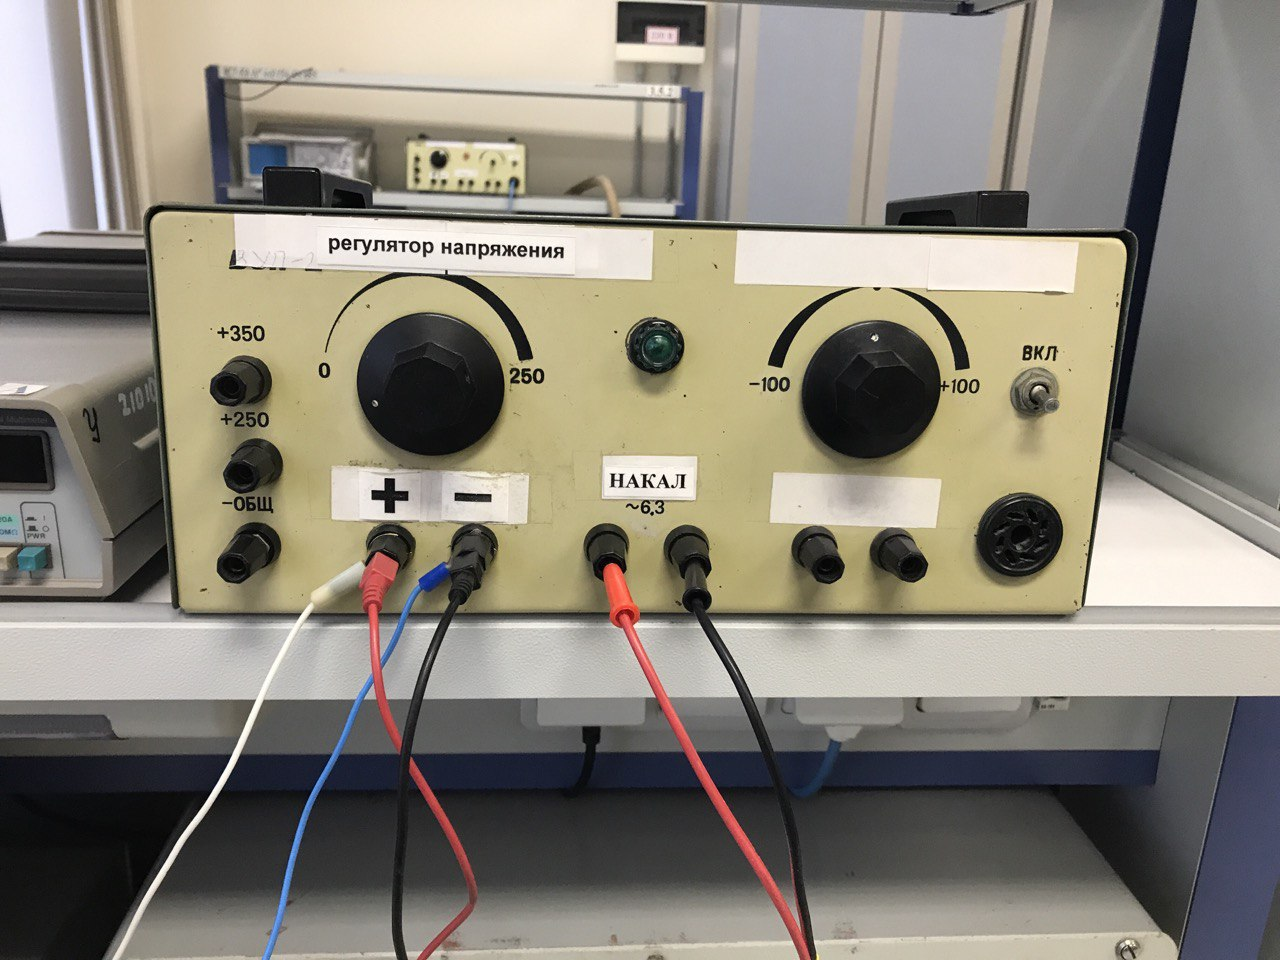
\includegraphics[scale={0.2}]{блок.jpg}

\end{center}

\section{Проверка работоспособности}

\noindent Определим с помощью осциллографа частоту напряжения, создаваемого генератором, - она составляет примерно 10 МГц.

\medskip
\begin{center}

  \centering
  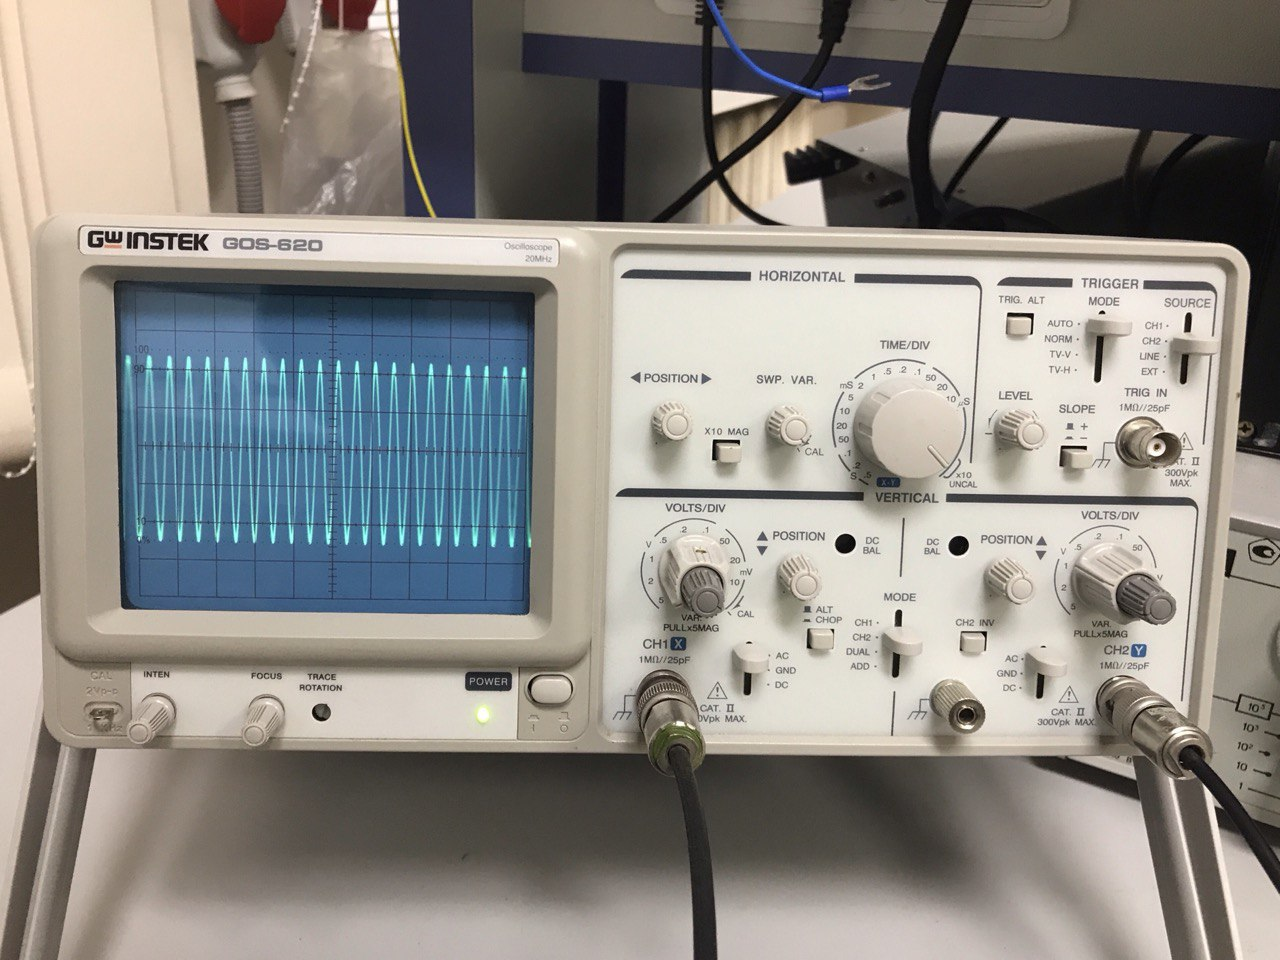
\includegraphics[scale={0.2}]{осц.jpg}


\end{center}

\noindent Предполагалось, что при подключении схемы к источнику будем наблюдать искру - электрический разряд ярко-голубого цвета. Этого не происходит из-за недостаточного значения напряжения, создаваемого генератором.

\medskip

\noindent Также предполагалось провести опыт с неоновой лампочкой: при поднесении на расстояние нескольких сантиметров к верхней части катушки $L_3$ она должна была светиться. Это свечение говорит о том, что напряженность электрического поля в разреженном неоне, заполняющем лампочку, вблизи генератора превышает критическое значение, при котором наступает электрический пробой газа. 

\medskip

\noindent Разумеется, при контакте неоновая лампочка загорается. 

\medskip
\begin{center}

  \centering
  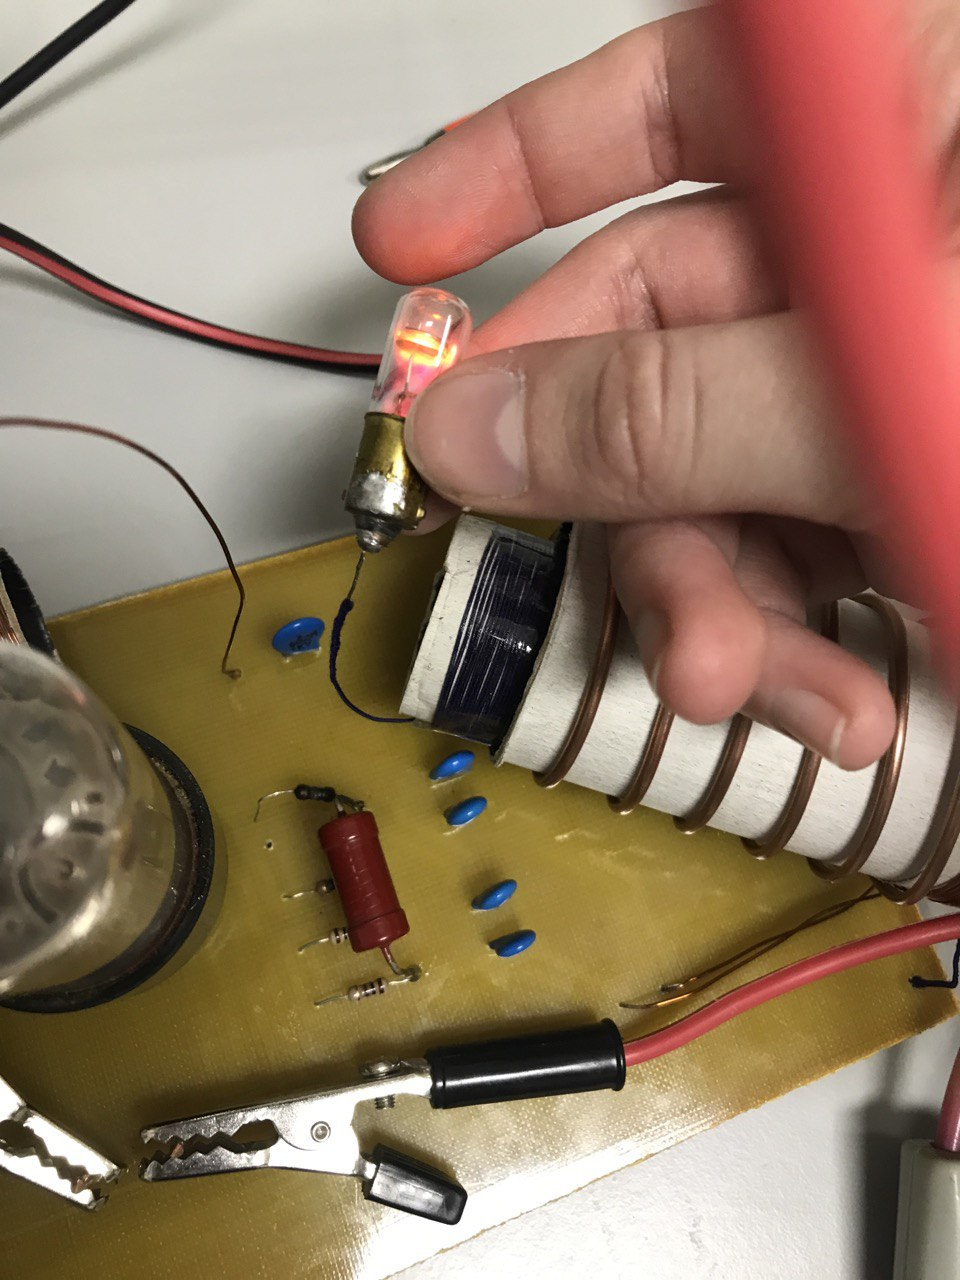
\includegraphics[scale={0.2}]{неон.jpg}


\end{center}

\noindent Предположительно, недостаточное для пробоя напряжение связано с ошибкой в числе витков катушек.

\end{document}